\subsection{Tipo de entidad Matrícula}

   \begin{description}

   \item[Definición] Se refiere al objeto del mundo real: \emph{``Registro de un
   alumno en una determinada asignatura como resultado de la matriculación''}.

   \item[Características] La entidad presenta las siguientes características:
      \begin{itemize}
         \item \textbf{Nombre:} Matrícula.
         \item \textbf{Tipo:} Débil por identificación con respecto a las
         entidades Alumno Curso Académico y Asignatura Curso Académico.
         \item \textbf{Número de atributos:} 1 propio y 5 heredados.
         \item \textbf{Atributo/s identificador/es principal/es:} dni\_pasaporte
         junto con curso\_académico, id\_centro, id\_titulación e id\_asignatura.
         \item \textbf{Atributo/s identificador/es alternativo/s:} -
         \item \textbf{Atributo/s heredado/s:} dni\_pasaporte y curso\_académico
         del tipo de entidad Alumno Curso Académico, junto a los atributos id\_centro,
         id\_titulación, id\_asignatura y curso\_académico, que se heredan del
         tipo de entidad Asignatura Curso Académico.
         \item \textbf{Información adicional:} El atributo curso\_académico del
         tipo de entidad Asignatura Curso Académico no se representa ya que se
         está representando el atributo del mismo nombre del tipo de entidad
         Alumno Curso Académico y que representa, forzosamente, la misma
         información. También es necesario destacar que, mediante la lógica del
         sistema, se deberá comprobar que para cada curso académico, solo es
         posible establecer la calificación de dos convocatorias, ya que es el
         máximo permitido por la normativa vigente.
      \end{itemize}

   \item[Diagrama] La figura \ref{diagramaMatricula} muestra el diagrama de la entidad.
   \item \begin{figure}[!ht]
            \begin{center}
            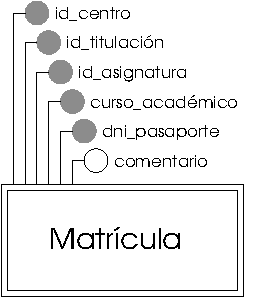
\includegraphics[]{07.Modelo_Entidad-Interrelacion/7.2.Analisis_Entidades/diagramas/matricula.pdf}
            \caption{Diagrama de la entidad Matrícula.}
            \label{diagramaMatricula}
            \end{center}
         \end{figure}

   \item[Descripción de los atributos propios] La entidad presenta el
   siguiente atributo propio:

   \begin{itemize}
    \item \textbf{comentario}
    \begin{itemize}
      \item \textbf{Definición:} Información extra que pueda ser
      interesante conocer.
      \item \textbf{Dominio:} Conjunto de caracteres alfanuméricos.
      \item \textbf{Carácter:} Opcional.
      \item \textbf{Ejemplo práctico:} Prácticas superadas.
      \item \textbf{Información adicional:} El dato lo introduce el
      usuario alumno al actualizar su información personal , o
      bien el usuario asesor si comprueba que la información no es
      correcta.
    \end{itemize}
   \end{itemize}

   \item[Ejemplo práctico]

   \item \begin{center}
            \begin{tabular}{ | l | l | }
            \hline
            \multicolumn{2}{ | c | }{\textbf{Tipo de entidad Matrícula}} \\
            \hline
            dni\_pasaporte & 01234567A \\
            \hline
            curso\_académico & 2008 \\
            \hline
            id\_centro & 15 \\
            \hline
            id\_titulación & 3\\
            \hline
            id\_asignatura & 17\\
            \hline
            comentario & Prácticas superadas \\
            \hline
            \end{tabular}
         \end{center}
   \end{description}
